\BiChapter{深度置信网络}{DBN}\label{chapter:DBN}
深度置信网络是由Hinton于2006年提出的一种深度全连接神经网络,全连接的深度神经网络的训练是及其困难的,然而在深度置信网络中,我们采用网络的逐层训练,随后对网络参数的微调,这种策略使得我们可以容易地训练多层神经网络。由于深度置信网络本质是一种传统神经网络的推广,在本章中,我们将从传统神经网络说起,介绍其训练方法,逐步将其推广到深度置信网络。
\BiSection{神经网络组成及表达能力}
x一个神经网络往往由多层神经元组成,神经元作为网络的基本单元,在给定恰当的激活函数和权值的前提下,只要这个网络足够庞大,足以容纳较多的神经元,那么这个网络可以表达任何一个连续函数\citeup{barron1993universal},当然这只是一个理论上成立的理想情况,实际工程中,我们没有办法利用神经网络来描述所有的函数,但是这个定理能使我们对神经网络的表达能力充满信心。
\BiSubsection{神经元}
x一个神经元如图\ref{img:NNnode_cp5} 所示,它包含$d$个输入$x = [x_1, x_2\cdots, x_d]^T$以及对应的$d$个权值$w = [w_1, w_2\cdots, w_d]^T$,还有一个偏置$b$。此外,它还应包括一个执行非线性映射的激活函数$f(~\cdot~)$
\begin{figure}[!htbp]
\centering
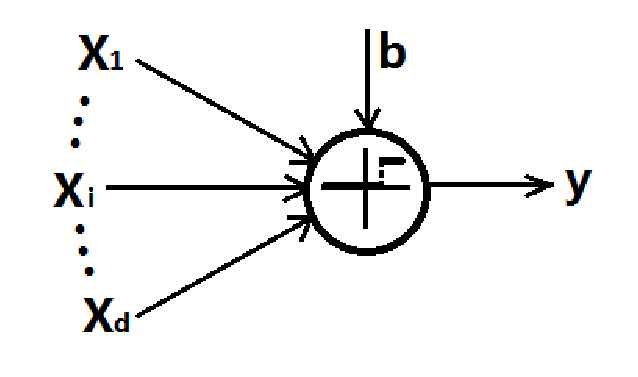
\includegraphics[width=0.33\textwidth]{DBN/NNnode.eps}
\caption{神经元}
\label{img:NNnode_cp5}
\end{figure}

与$d$个输入$x = [x_1, x_2\cdots, x_d]^T$直接相连的是数据的输入,例如,一章$28\times 28$像素的灰度图像作为网络输入,由于该图像可以展开成$28\times 28 = 784$的列向量,因此这个例子中的神经元就应该有784个输入,即$x = [x_1, x_2\cdots, x_{784}]^T$。$d$个权值$w = [w_1, w_2\cdots, w_d]^T$,刻画了$d$个输入$x = [x_1, x_2\cdots, x_d]^T$的重要性,$w$中的某个分量$w_i$越大,说明对应的分量$x_i$对最后决策结果的影响越大。从生物学的角度上看,$x$相当于给予生物各种刺激,$w$相当于该生物对各种刺激的敏感度。
例如,我们利用神经元设计一个医学诊断系统来判定一个人是否需要住院观察,对于该神经元,假设输入为$x = [\text{心脏疼痛},\text{头疼},\text{腰疼}]$,如果有某个症状,则对应位置1,否则置0。显然,若一个人心脏疼痛,我们更倾向于让他住院观察,因此我们为心脏疼痛对应的权值设定一个较大的权值$w_1 = 0.9$,头疼次之,我们设定为$w_2 = 0.5$,当一个人腰疼时,不太可能需要住院治疗,我们为其设定一个较小的偏置$w_3 = 0.1$。因此,这个神经元的权值为
\begin{equation}
w = [0.9, 0.5, 0.1]^T
\end{equation}

假设现在有一位患者来到医院,他既有头疼又有心脏疼痛的症状,那么这位患者可以表示为向量
\begin{equation}
x = [1, 0, 1]^T
\end{equation}
此时,病情积累的严重性为
\begin{equation}
w^Tx = 0.1+0.9 = 1
\end{equation}
那么这位患者是否需要住院呢?为此,我们利用前面提及到的偏置$b$来刻画这件事。假设$b = 0.7$,如果$w^Tx>b$,则说明这位患者患有严重的疾病,需要住院观察,网络输出$y=1$,否则这位患者不需要住院,网络输出$y=0$。如果我们定义为神经元的净激活为
\begin{equation}
net = w^Tx + b
\end{equation}
净激活可以理解为排除偏置干扰后神经元接收到的刺激总和。那么上述判别过程相当于用一个阶跃函数对净激活作一个非线性映射,即
\begin{equation}
y = f(net) = \left\{
\begin{array}{cc}
1 & \text{若}w^Tx - b> 0 \\
0 & \text{其他}
\end{array}
\right.
\end{equation}

其中,由于$b$是一个常数,因此$w^Tx +b$与$w^Tx - b$并没有区别。但实际上,$b = 0.7$时的神经元做出的决策,其结果只由心脏疼痛这个因素决定,因为如果一个患者没有心脏疼痛,那么最大的净激活是在他即患有头疼又患有腰疼的情况下取得,此时$net=0.6$。而$0.6<0.7$,并不会让他住院。因此,上面的神经元,转换成等价的逻辑命题便是:如果一个人的症状中含有心脏疼痛,则需要住院,否则不需要住院。如果我们把偏置调低,另$b=0.55$,则此时等价的逻辑命题为:如果一个人的症状中含有心脏疼痛,或者症状中既含有头痛有含有腰疼,则需要住院,否则不需要住院。综合以上讨论,偏置起到的是阈值的作用,但是这个阈值取多少就是设计者的意愿了,不同的阈值一般情况下会等价于不同的逻辑命题,这取决于系统的期望输出是什么。

神经元总能转换成一个对应的逻辑表达,需要提出的一个因果关系是,我们并不是从逻辑表达中推出神经元的参数,而是从神经元的参数中可以得到一个逻辑表达。神经元的优点在于,通过一个神经元,便可以实现一个简单的决策,如果拥有更多的神经元,将他们组合起来形成一个神经网络,便可以实现更为复杂的决策行为。这个决策的因果关系是由参数决定的,后面我们将会看到,参数是通过统计学习学到的,因此在神经网络中,我们不需要对事物的因果关系进行分析,只需要使用大量的数据让网络学习其中的因果关系,这些因果关系对于我们而言是透明的。


\BiSubsection{逻辑表达}
x在本小节,我们将再一次讨论网络的逻辑表达能力,如图\ref{img:NNnodeXY.png} 所示的一个接收两维输入的神经元,其偏置$w = [-2, -2]^T$,偏置$b=3$

\begin{figure}[!htbp]
\centering
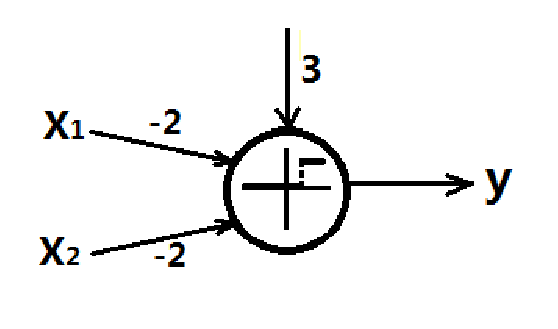
\includegraphics[width=0.33\textwidth]{DBN/NNnodeXY.eps}
\caption{与非门的神经元表达}
\label{img:NNnodeXY.png}
\end{figure}

如果我们的输入至少有一个为假,即$x = [0,0]^T$或$x = [1,0]^T$或$x = [0,1]^T$,则网络的输出为真,即$y=1$,若两个输入都为真,即$x = [1,1]^T$,则网络的输出为假,即$y=0$。事实上,图\ref{img:NNnodeXY.png}等价于逻辑电路中的与非门,即
\begin{equation}
y = \overline{ x_1\cdot x_2}
\end{equation}
由于与非门是通用们,可以利用多个与非门构建出三大逻辑门:与门、或门、非门。因此,利用图\ref{img:NNnodeXY.png}中的神经元可以表达任意一个逻辑函数。例如,在半加器中,其逻辑函数为
\begin{equation}
y_1 = x_1 \oplus x_2
\end{equation}
\begin{equation}
y_2 = x_1 \cdot x_2
\end{equation}
利用与非门搭建的电路图如图\ref{img:numberHalfAdd}所示,而将其转换成对应的神经网络如图\ref{img:NNhalfAdd}所示\footnote{图中,为了美观,我们并没有将偏置画出来}。

\begin{figure}[htbp]
\centering
\subfigure{\label{img:numberHalfAdd}}\addtocounter{subfigure}{-2}
\subfigure{\subfigure[由与非门搭建的半加器]
			{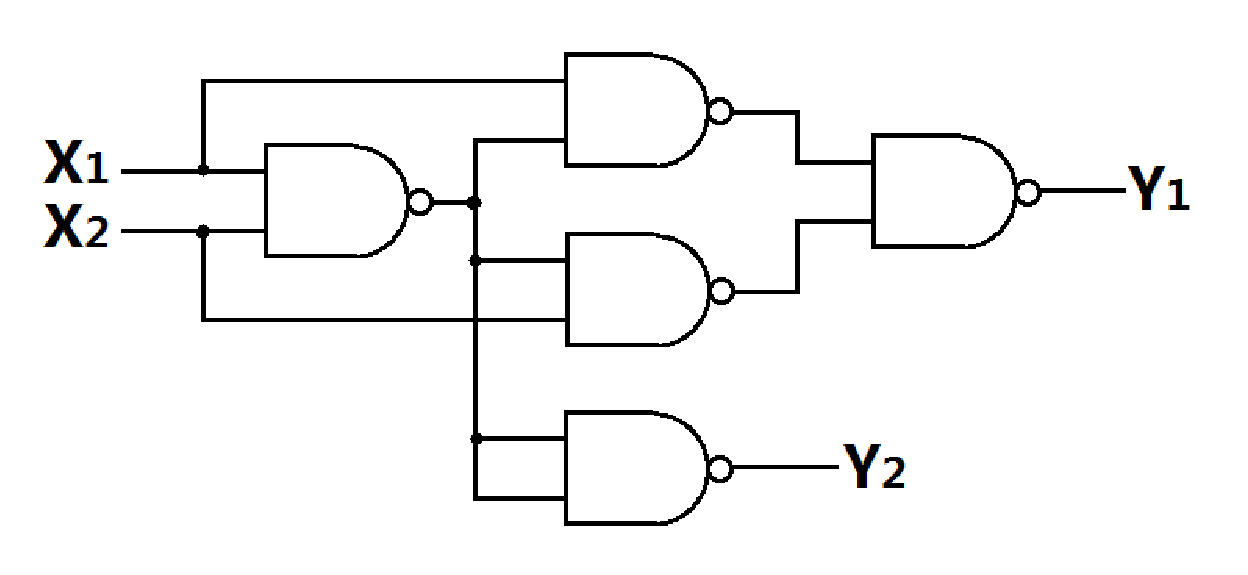
\includegraphics[width=0.5\textwidth]{DBN/numberCirc.eps}}}
\subfigure{\label{img:NNhalfAdd}}\addtocounter{subfigure}{-2}
\subfigure{\subfigure[由神经元搭建的半加器]
			{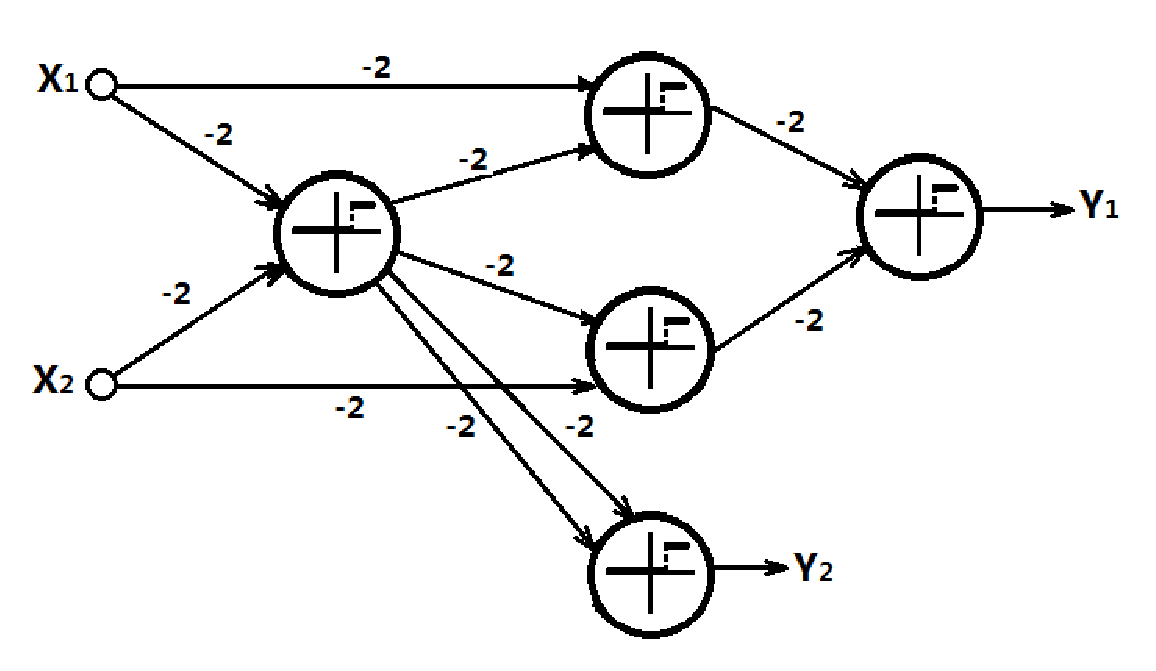
\includegraphics[width=0.4\textwidth]{DBN/NNCirc.eps}}}
\caption{半加器的两种不同描述}
\label{img:halfAdd}
\vspace{-1em}
\end{figure}

我们之所以花费篇幅去介绍神经元的表达能力,是为了说明神经网络确实能实现一些逻辑决策,但并不意味着网络的权值需要我们手工设定的。这里的权值之所以要手工设定,是因为我们精心筛选出来用以阐述神经网络的表达能力,但实际应用中,权值是通过误差传播自动学习的,学习到的权值,其对应的逻辑命题对于人类而言是难以理解的,但这并不重要,因为我们需要的是仅仅决策结果,而不是这个决策是如何产生的因果关系。

\BiSection{神经网络的前馈}
x一般而言,神经网络是一个多层结构组织,网络的每一层都由多个神经元阻生,上一层的神经元由下一层的神经元激活。同一层的神经元之间没有连接,因此同一层节点的激活是独立的。神经网络接收到一个数据后,逐层地激活各层的神经元,下一层的输出作为上一层的输入,最后得到一个输出结果。这个过程称为神经网络的前馈或前向传播。

\begin{figure}[!htbp]
\centering
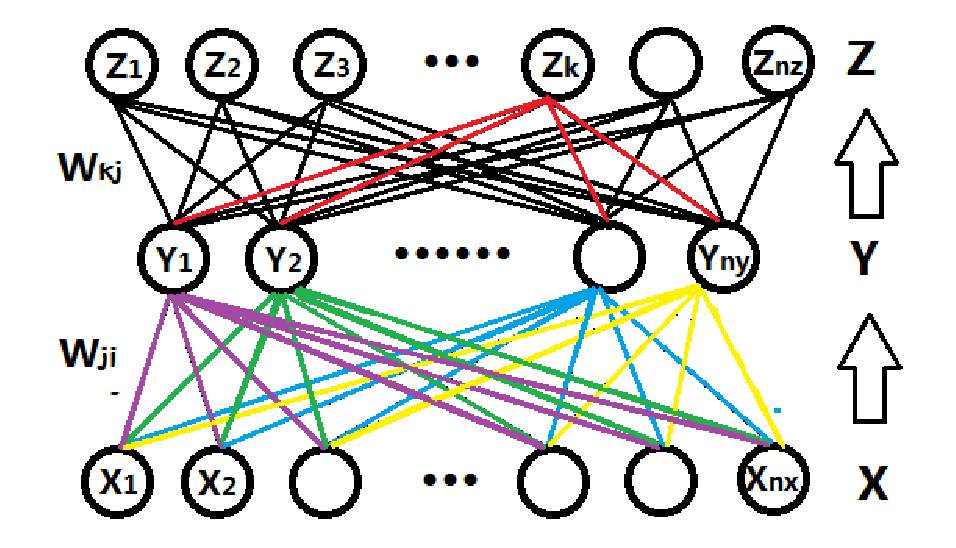
\includegraphics[width=0.55\textwidth]{DBN/3NNfp.eps}
\caption{神经网络的前馈}
\label{img:3NNfp}
\end{figure}

如图\ref{img:3NNfp}所示是一个三层神经网络,由于神经激活是自底向上传播的,如果各层的激活函数都相同,为$f(~\cdot~)$,则网络的第k个节点的输出为
\begin{equation}
z_k = f\bigg[\sum\limits_{j=1}^{n_y} w_{kj} 
f(\sum\limits_{i=1}^{n_x} w_{ji}) + b_j)
+ b_k\bigg]
\label{equ:DBN_NNoutput}
\end{equation}
式中,$w_{kj} $为$y$层的第$j$个节点到$z$层的第$k$个节点之间的连接权值,$w_{ji} $为$x$层的第$i$个节点到$y$层的第$j$个节点之间的连接权值,$b_j$为$y$层第$j$个节点的偏置,$b_k$为$z$层第$k$的节点的偏置。

神经网络的这种自底向上的激活,有时也被解释为特征提取或重新编码。当接收到一个数据时,神经网络将这个数据逐层地进行特征抽取,过滤掉一些冗余信息,将剩余的重新编码,最后利用一个分类器将抽取到的最抽象(即最顶层)特征进行分类,从而完成整个识别过程。

\BiSubsection{神经激活}
x到目前为止,我们只介绍了一种激活函数,即阶跃函数,但实际中我们并不会使用阶跃函数作为激活函数。首先,阶跃函数是不连续的,其次,阶跃函数是不可导的\footnote{事实上阶跃函数是可导的,其导函数为脉冲函数,这是一个广义函数,我们不深入讨论}。激活函数不可导,将导致网络无法利用反向传播进行训练,关于这点我们将在反向传播章节讨论。作为激活函数,它应该满足以下几个条件
\begin{enumerate}
\item 它必须是非线性的。由式\eqref{equ:DBN_NNoutput}可以看出,若激活函数是线性的,则多层神经网络实际上只相当于两层网络,因为多个矩阵相乘的结果为一个矩阵。网络一旦失去多层结构,则表达能力迅速下降。
\item 它应该具有饱和特性,即至少存在一个上界或下界。饱和特性的存在,使得神经元的输出不至于过高或过低,整个网络的编码维持在一定的范围内。但最近的研究表明,一些近似饱和的激活函数也能工作得很好,如此看来,饱和似乎并不是必要的,但近似饱和还是需要的。
\item 它应该连续且可导。由于反向传播中需要求取激活函数相对于净激活的偏导数,如果激活函数是不可导的,那么反向传播算法将无法执行。
\end{enumerate}
实际工程中,我们常用的激活函数是sigmoid函数\footnote{也被称为logistic函数}或双曲正切函数。其中,sigmoid函数我们定义为
\begin{equation}
f(net) = \frac{1}{1+ e^{-net}}
\end{equation}
其对应的图像如图\ref{img:sigmoid}所示
\begin{figure}[!htbp]
\centering
\includegraphics[width=0.5\textwidth]{DBN/sigmoid.eps}
\caption{sigmoid激活}
\label{img:sigmoid}
\end{figure}

可以看到,sigmoid函数是一个值域为$(0,1)$的连续可导函数,其导函数有一个重要特性,即
\begin{equation}
\begin{split}
f'(net) &= \frac{e^{-net}}{(1 + e^{-net})^2} = \frac{1}{1+ e^{-net}} -  \frac{1}{(1+ e^{-net})^2}\\
&=f(net)\Big[1 - f(net)\Big]
\end{split}
\label{equ:logisticDiff}
\end{equation}

这个特性之所以重要,是应为利用式\eqref{equ:logisticDiff}可以直接通过网络的输出直接计算激活函数相对于净激活的偏导数而不必引入额外的计算。我们看到,sigmoid函数的输出范围为$(0,1)$,有时候,我们希望网络的输出为$(-1,1)$,此时可以使用双曲正切函数,即
\begin{equation}
f(net) = \tanh(net) = \frac{e^{net} - e^{-net}}{e^{net} + e^{-net}}
\end{equation}
其对应的图像如图\ref{img:tanh}所示
\begin{figure}[!htbp]
\centering
\includegraphics[width=0.5\textwidth]{DBN/tanh.eps}
\caption{tanh激活}
\label{img:tanh}
\end{figure}

近年来,在神经网络的研究上又提出了一些新的激活函数,其中最重要的莫过ReLU激活函数,其定义为\citeup{glorot2011deep}
\begin{equation}
f(net) = \left\{
\begin{array}{cc}
net & \text{若}net > 0\\
0 & \text{其他}
\end{array}
\right.
\label{equ:ReLU}
\end{equation}
式\eqref{equ:ReLU}也可以简写为
\begin{equation}
f(net) = \max (0, net)
\end{equation}
其对应的图像如图\ref{img:ReLU}所示
\begin{figure}[!htbp]
\centering
\includegraphics[width=0.48\textwidth]{DBN/ReLU.eps}
\caption{ReLU激活}
\label{img:ReLU}
\end{figure}

这种激活函数相比于sigmoid函数有较大的改进,关于其优点我们将留到反向传播的章节讨论。但ReLU有一个缺点:在$net<0$时导数为0,从而导致反向传播无法更新参数。因此,在ReLU的基础上又产生了一些变体,例如,softplus中,激活函数定义为\citeup{glorot2011deep}
\begin{equation}
f(net) = \log(1+e^{net})
\end{equation}
其对应的图像如图\ref{img:softplus}所示
\begin{figure}[!htbp]
\centering
\includegraphics[width=0.48\textwidth]{DBN/softplus.eps}
\caption{softplus激活}
\label{img:softplus}
\end{figure}

从图中不难看出,softplus是ReLU的圆滑版,关于softplus,一个有意思的结论是,其激活函数的导数为logistics函数,即
\begin{equation}
f'(net) = \frac{e^{net}}{1 + e^{net}} = \frac{1}{1 + e^{-net}}
\end{equation}
然而这个结论并没有什么用处,因为它并不能减轻程序的计算量。

ReLU的另一种变体是由He Kaiming等人提出的PReLU,其激活函数定义为\citeup{MS2015}
\begin{equation}
f(net) = \left\{
\begin{array}{cc}
net & \text{若} net >0\\
\alpha net & \text{若} net \leq 0
\end{array}
\right.
\end{equation}
式中,$\alpha$为一个较小的参数,例如当$\alpha = 0.1$时,其图像如图\ref{img:PReLU}所示
\begin{figure}[!htbp]
\centering
\includegraphics[width=0.5\textwidth]{DBN/PReLU.eps}
\caption{PReLU激活}
\label{img:PReLU}
\end{figure}

显然,PReLU在负半平面不再会出现导数为0的情况。尽管参数$\alpha$需要学习得到,但这种方法在ImageNet 2012数据集上获得了非常好的识别效果,首次在图像识别任务上超越了人的识别效果,错误率仅为4.94\%。在该文中,作者提到了一个有意思的现象:在较低层的网络中,学习到的参数$\alpha$较大,而在高层的网络中,参数$\alpha$较小。作者的猜测是较低曾网络需要尽可能多地保留数据的信息,因此激活函数更倾向于类线性,而高层网络更倾向于抽象数据的结构,从而做出决策,因此高层的激活函数更倾向于非线性。

在同一个任务中,激活函数的不同选取会有不同的实验现象,目前并没有证明哪种激活函数更好。习惯上,在全连接神经网络中,我们更喜欢sigmoid派的激活函数,而在卷积网络中,我们更喜欢ReLU派的激活函数,尽管这些都不是强制的。


\BiSection{分类器}
x神经网络的逐层激活,其本质在于将一种编码转化成另一种编码。编码之间的转换,可以过滤掉一些原始编码中无用的噪声或信息,这个过程一般都伴随着熵的减小(但并不绝对)。然而,一个神经网络在最顶层的激活,其编码是人类所无法理解的,因此,在最顶层节点之上还需要一个分类器对神经网络提取到的特征或者说编码进行分类。分类器其作用,一方面在于将编码转换为人类所能理解的编码,这在有监督的分类任务以及无监督的聚类任务中是必要的,因为我们最后希望网络能给我们一个输出标签。但对于降维任务而言有时候并不是必要的,因为降维并不需要输出标签。另一方面,分类器都带有一个准则函数,这个准则函数定义了熵,即定义了什么是混乱,什么是有序。从控制论的角度上看,控制工程中,误差是系统校正的核心,没有误差便没有反馈,没有反馈,则系统难以控制。机器学习也是同样的道理,没有误差,则无法对参数进行校正,机器便无法从样本中学习。误差的来源,源自于准则的定义,即预先预定什么是对的,什么是错的,对于错之间就会存在一个误差,如果机器产生了一个误差,利用这个误差便可以对参数进行校正。神经网络冲,常用的分类器有三种:平方误差、softmax、支撑向量机,尽管支撑向量机是一种重要的分类器,但是鉴于篇幅有限,我们并不打算在本文中介绍支撑向量机,关于其原理读者可参考文献xxxx。

\BiSubsection{平方误差分类器}
x严格来说,平方误差并不能算作一个分类器,它充其量只能算作一个准则,这个准侧除了在神经网络中有应用之外,在很多领域也有广泛的应用。平方误差,或者说二范数,其准则函数定义为
\begin{equation}
L = \sum\limits_{i=1}^d (x_i -t_i)^2
\label{equ:L2error}
\end{equation}
式中,$x_i$为网络的输出,这个输出由输入数据与网络参数共同决定,$t_i$代表标签值,也成为教师信号,由数据的标签值决定,$d$则是$x$的维数。假设一个神经网络的最顶层有4个节点,网络的输出为$[~-0.1~~0.1~~0.8~~0.1~]$,而我们的期望输出是$[~0~~0~~1~~0~]$(再一次强调,这个期望输出由标签值决定),那么实际输出与期望输出之间就会存在一个误差向量$[~-0.1~~0.1~~0.2~~0.1~]$,将其转化成平方误差后为$[~0.01~~0.01~~0.04~~0.01~]$,利用式\eqref{equ:L2error}可以很容易算的此时$L=0.07$。事实上,$L=0.07$对我们而言没有太大用处,它最多只能刻画总的误差量有多大,真正对我们有用的是平方误差向量,利用这个向量,可以将误差反向传播回神经网络的底层,从而自顶向下就网络参数进行校正,关于这个过程更多的细节,我们将会留到反向传播章节介绍。

\BiSubsection{softmax分类器}
x实际中,为了方便分类,我们往往希望网络的输出是“k中取1”的形式,例如,假设我们有四个类别,如果使用二进制编码的话,我们只需两个节点即可,即00代表第一类,01代表第二类,以此类推。如果我们使用所谓的“k中取1”形式,我们便需要四个节点,即0001代表第一类,0010代表第二类,0100代表第三类,1000代表第四类。为了实现“k中取1”的形式,我们需要引入softmax分类器,softmax分类器可以认为是logistics回归的推广,在使用logistics回归进行分类时,只能实现两类分类,而softmax分类器可以实现多类分类功能。

在softmax分类器中,假设容量为$n$的训练集为$S = \big\{(x^{(1)}, y^{(1)}), \cdots, (x^{(n)}, y^{(n)})\big\}$,由于标签$y$的取值可以有$c$种,因此$y^{(i)} \in \{1, 2,  \cdots, c\}$。我们引入记号$(\phi_1, \phi_2, \cdots, \phi_c)$来表示各个类别的输出概率,由于$\sum\phi_i = 1$,因此记号存在冗余,只需要$c - 1$个记号$(\phi_1, \phi_2, \cdots, \phi_{c-1})$即可,对于$\phi_i$,有
\begin{equation}
\phi_i = P(y = 1; \phi)
\end{equation}
以及
\begin{equation}
\phi_c = P(y = c; \phi) = 1 - \sum\limits_{i=1}^{c-1}\phi_i
\end{equation}
注意,正如我们之前提到的,$\phi$中参数存在冗余,所以$\phi_c$并不是参数,而是一个为了方便后面讨论所引入的一个记号。

由于softmax的概率分布也属于指数分布族,而在指数分布族中,对于概率分布而言,都可以写成如下形式
\begin{equation}\label{equ:expFamily}
P(y; \eta) = b(y) \exp \bigg[\eta^T T(y) - a(\eta)\bigg]
\end{equation}

在softmax中,我们记$T(y) \in R^{c-1}$为

\begin{equation}
T(1) = \left[               %左括号
\begin{array}{cccc}  
1\\  
0\\
\vdots\\
0
\end{array}
\right]~~~~%%%%%%%%%%%%%%%%%%%%
T(2) = \left[   
\begin{array}{cccc}  
0\\  
1\\
\vdots\\
0
\end{array}
\right]~~~~~~%%%%%%%%%%%%%%%%%%%
\cdots~~~~~~
T(c-1) = \left[   
\begin{array}{cccc}  
0\\  
0\\
\vdots\\
1
\end{array}
\right]~~~~%%%%%%%%%%%%%%%%
T(c) = \left[   
\begin{array}{cccc}  
0\\  
0\\
\vdots\\
0
\end{array}
\right]~~~~%%%%%%%%%%%%%%%%%%%%%% 
\end{equation}
记$\Big[T(y)\Big]_i$为$T(y)$的第$i$个元素,记$1 \{\cdot\}$为示性函数,即
\begin{equation}
1 \{A\} = \left\{
\begin{array}{cc}
1 & \text{,若命题$A$为真} \\
0 & \text{,若命题$A$为假}
\end{array}
\right.
\end{equation}
因为$\Big[T(y)\Big]_i = 1\{y = i\}$,因此
\begin{equation}
\begin{split}
\mathbb{E}\bigg[\big[T(y)\big]_i\bigg] &= \big[T(y)\big]_i \cdot P(y = i) \\
&= P(y=i)  \\
&= \phi_i
\end{split}
\end{equation}

而
\begin{equation}
\begin{split}
P(y; \phi) &= \phi_1^{1\{y=1\}} \phi_2^{1\{y=2\}}\cdots\phi_c^{1\{y=c\}} \\
&=\phi_1^{1\{y=1\}} \phi_2^{1\{y=2\}}\cdots\phi_c^{1 - \sum\limits_{i=1}^{c - 1}1\{y = i\}} \\
&=\phi_1^{\big[T(y)\big]_1}\phi_2^{\big[T(y)\big]_2}\cdots\phi_c^{1 - \sum\limits_{i=1}^{c-1}\big[T(y)\big]_i}\\
&=\exp\bigg\{\ln\Big[\phi_1^{\big[T(y)\big]_1}\phi_2^{\big[T(y)\big]_2}\cdots\phi_c^{1 - \sum\limits_{i=1}^{c-1}\big[T(y)\big]_i}\Big]\bigg\} \\
&=\exp\bigg\{ \Big[T(y)\Big]_1\ln\phi_1 + \Big[T(y)\Big]_2\ln\phi_2+\cdots + \bigg[1-\sum\limits_{i=1}^{c-1}\Big[T(y)\Big]_i \bigg]\ln\phi_c \bigg\}\\
&=\exp\bigg\{\Big[T(y)\Big]_1\ln\frac{\phi_1}{\phi_c} + \Big[T(y)\Big]_2\ln\frac{\phi_2}{\phi_c} + \cdots  +  \ln \phi_c \bigg\}
\end{split}
\end{equation}
对比式\eqref{equ:expFamily},得
\begin{equation}
b(y) = 1
\end{equation}
\begin{equation}
\eta = \Big[~~\ln\frac{\phi_1}{\phi_c}~~~~\ln\frac{\phi_2}{\phi_c}~~~~\cdots~~~~\ln\frac{\phi_{c-1}}{\phi_c}~~\Big]^T
\end{equation}
\begin{equation}
a(\eta) = -\ln\phi_c
\end{equation}
定义
\begin{equation}
\eta_i = \ln\frac{\phi_i}{\phi_c}~~~~~~~~\eta_c = \ln \frac{\phi_c}{\phi_c}=0
\end{equation}
由于
\begin{equation}
e^{\eta_i} = \frac{\phi_i}{\phi_c}
\end{equation}
则
\begin{equation}
\phi_c\cdot e^{\eta_i} = \phi_i
\end{equation}
且
\begin{equation}
\phi_c\sum\limits_{i=1}^c e^{\eta_i}= \sum\limits_{i=1}^c \phi_c e^{\eta_i}
=\sum\limits_{i=1}^k\phi_i
=1
\end{equation}
从而
\begin{equation}
\phi_i = \phi_c e^{\eta_i} = \frac{\exp(\eta_i)}{\sum_{i=1}^c \exp(\eta_i)}
\end{equation}
即
\begin{equation}
P(y=i;\phi) = \phi_i =\frac{\exp(\eta_i)}{\sum_{i=1}^c \exp(\eta_i)}
\end{equation}
以及
\begin{equation}
P(y=i|x;\theta) = \frac{\exp(\theta_i^Tx)}{\sum_{j=1}^c\exp(\theta_j^T x)}
\end{equation}

本质上,softmax分类器都可以看做是一种两层神经网络,与常规的神经网络中使用sigmoid函数作为激活函数不同,在softmax分类器中,激活函数$f(net_k) \propto e^{net_k}$,对应的激活概率定义为\citeup{Duda}
\begin{equation}\label{temp3}
z_k = \frac{e^{net_k}}{\sum_{i=1}^c e^{net_i}}
\end{equation}
式中,$z_k$代表第$k$个节点激活的概率,$net_k$代表第$k$的节点的净激活,取值为输入特征$x$的线性函数,即$net_k = \theta_k  x^T$,$c$为类别的总数。在式\eqref{temp3}中分母的作用下,我们对每个类别的输出都进行了归一化,所以总的激活概率为1。在识别中,计算各个类别的激活概率后,只需选取最大激活概率所对应的类别作为输出类别即可。

\BiSection{神经网络的反馈}
x神经网络的反馈是基于准则函数的反馈,准则函数作为误差的度量,刻画了网络的输出与训练集的标签两者之间的差异。整个反馈过程中,实质上就是准则函数最小化的过程,即对网络的参数进行更新,使得误差不断减小。假设一个以参数$\theta$为自变量的准则函数$f(\theta)$,反馈过程就相当于不断寻求$\theta$使得$f(\theta)$最小的过程。如果$f(\theta)$是凸的,即Hessian矩阵是正定的,那么我们称这个问题为凸优化问题,我们可以有很多策略解决凸优化问题,但实际中遇到的问题基本都是非凸问题,解决非凸问题,一个简单有效的方法是利用梯度下降。想象我们在一座山上,为了更快速的下山,我们可以每一步都朝着当前最陡峭的方向(即梯度方向)前进,梯度下降也是基于这个原理,每一次迭代,我们都在当前的$\theta$下计算$f(\theta)$的梯度$\Delta_\theta f(\theta)$,让$\theta$加上这个梯度分量,也就是让它朝着梯度下降的方向迭代。由于梯度下降的每一步都是基于当前的参数$\theta$,所以这是一个贪婪算法,并不能保证收敛到全局最优。如果$f(\theta)$是凸的,那么梯度下降在大部分情况下它会收敛到全局最优(但并不绝对),然而,实际任务由于其非凸性,我们基本上不可能收敛到全局最小值,我们得到的往往是局部极小值。另外,值得一提的是,收敛到全局最小值是没有意义的,因为这个全局最小值是基于训练集的最小值,一旦收敛到此处,意味着网络可以很好地刻画训练集,但并不意味它同样可以很好地泛化到测试集上,这个时候往往会伴随着较高的过拟合风险,我们不应一味地最求全局最小,而应在训练集与测试集两者之间进行一个权衡。梯度下降,因其简单有效的特点,称为优化问题中一个很常用的策略。
\BiSubsection{分类器参数校正}
x20世纪80年代以前,人们并没有找到一个较好的方法训练神经网络,这种状况一直维持到1986年,在这一年里由Rumelhart与Mecelland为首的科学家小组\footnote{事实上反向传播是由很多人在同一年代同时独立提出的} 提出了方向传播算法,首次在神经网络中利用梯度下降逐层地训练网络参数,每训练完一层后将当前层的误差传递回下一层,依次迭代,最后完成整个网络的训练。在这套方法中,核心点有两个:如何利用最顶层(即分类器)的误差来更新最顶层的参数以及如何在某一层网络更新完参数后将该层的误差传播回前一层,我们将会在本小节中讨论最顶层的参数校正,并在下一小节讨论误差传播。
\BiSubsubsection{平方误差分类器参数校正}
x由于在平方误差分类器中,准则函数定义为
\begin{equation}
J(\theta) = \frac{1}{2}\sum\limits_{i=1}^c(t_i - z_i)^2 = \frac{1}{2}||t-z||^2
\end{equation}
式中,$z_i$为训练集的标签值,而网络的输出$t_i$又是由前一层的静激活经过非线性映射后得到的,即
\begin{equation}
t_i = f(net_i)
\end{equation}
式中,$net_i$为输出层的前一层,即倒数第二层的净激活,而这个净激活又被定义为
\begin{equation}
net_i = wx + b
\end{equation}
式中,$w$为输出层与倒数第二层两者之间的权值,$b$为偏置,因此,我们不难通过链式求导得到误差相对于参数的梯度,即$J(\theta)$相对于$\theta$(这里的$\theta$即为$w$和$b$)的导数
\begin{equation}
\frac{\partial J(\theta)}{\partial w} = \frac{\partial J(\theta)}{\partial net} \frac{\partial net}{\partial w}\label{equ:5.0}
\end{equation}
以及
\begin{equation}
\frac{\partial J(\theta)}{\partial b} = \frac{\partial J(\theta)}{\partial net} \frac{\partial net}{\partial b}\label{equ:5.00}
\end{equation}
如果此时的激活函数是sigmoid函数,那么容易知道
\begin{equation}
\frac{\partial J(\theta)}{\partial net} = net(1-net)\label{equ:5.1}
\end{equation}
如果激活函数是ReLU函数,也容易得到
\begin{equation}
\frac{\partial J(\theta)}{\partial net} = \left\{
\begin{array}{cc}
1 & \text{若}net>0\\
0 &\text{若}net\leq 0\\
\end{array}
\right.\label{equ:5.2}
\end{equation}
而$\partial net/\partial \theta$只是一个线性函数,同样容易求得
\begin{equation}
\frac{\partial net}{\partial w} = x~~~~~~~~\frac{\partial net}{\partial b} = 1\label{equ:5.3}
\end{equation}
利用\eqref{equ:5.1}或\eqref{equ:5.2}\footnote{这取决于你的激活函数选取}以及\eqref{equ:5.3}便可以求取式\eqref{equ:5.0}以及\eqref{equ:5.00}中参数应该修改的幅度,即梯度。






\BiSubsubsection{softmax分类器参数校正}
在softmax的训练中,由于我们的期望输出为
\begin{equation}
h_\theta(x) =\mathbb{E}\Big[T(y)|x;\theta \Big]
%%%%%%%%%%%%%%%%%%%%%%%%%%%
=\mathbb{E}\left[
\begin{array}{cccc}
1\{y=1\}\\
1\{y=2\}\\
\vdots\\
1\{y=c-1\}
\end{array}
\right | x; \theta
\left.
\begin{array}{cccc}\\\\\\\\\end{array}
\right]
%%%%%%%%%%%%%%%%%%%%%%%%%%%
=\left[
\begin{array}{cccc}
\phi_1\\
\phi_2\\
\vdots\\
\phi_{c-1}
\end{array}
\right] 
%%%%%%%%%%%%%%%%%%%%%%%%%%%
=\left[
\begin{array}{cccc}
\frac{\exp(\theta_1^T x)}{\sum_{j=1}^c \exp(\theta_j^T x)}\\
\frac{\exp(\theta_2^T x)}{\sum_{j=1}^c \exp(\theta_j^T x)}\\
\vdots\\
\frac{\exp(\theta_{c-1}^T x)}{\sum_{j=1}^c \exp(\theta_j^T x)}
\end{array}
\right]
\end{equation}
对应的似然函数为
\begin{equation}
\mathcal{L}(\theta) = \prod\limits_{i=1}^n P(y^{(i)}|x^{(i)}; \theta)
\end{equation}
对应的对数似然函数为
\begin{equation}\label{equ:softmaxErr}
\begin{split}
\ell(\theta) &= \sum\limits_{i=1}^n\ln P(y^{(i)}|x^{(i)}; \theta)\\
&=\sum\limits_{i=1}^n\sum\limits_{j=1}^c \ln \bigg(\frac{\exp(\theta_j^Tx^{(i)})}{\sum_{t=1}^c\exp(\theta_t^T x^{(i)})} \bigg)^{1\{y^{(i)} = j\}}\\
&=\sum\limits_{i=1}^n\sum\limits_{j=1}^c 1\{y^{(i)} = j\} \ln \bigg(\frac{\exp(\theta_j^Tx^{(i)})}{\sum_{t=1}^c\exp(\theta_t^T x^{(i)})} \bigg)
\end{split}
\end{equation}
式\eqref{equ:softmaxErr}的相反数也被称为交叉熵,在训练过程中充当准则函数,我们对其求导,有
\begin{equation}
\begin{split}
\frac{\partial \ell (\theta)}{\partial\theta_j} 
&=\sum\limits_{i=1}^n\sum\limits_{j=1}^c 1\{y^{(i)} = j\}\bigg[x^{(i)} - \frac{\partial}{\partial\theta_j}\ln \sum\limits_{t=1}^c \exp\big(\theta_t^T x^{(i)}\big)\bigg]\\
&=\sum\limits_{i=1}^n\sum\limits_{j=1}^c 1\{y^{(i)} = j\} \bigg[ x^{(i)} - \frac{\exp(\theta_j^T x^{(i)})}{\sum_{t=1}^c\exp(\theta_t^T x^{(i)})} x^{(i)}\bigg]\\
&=\sum\limits_{i=1}^n\sum\limits_{j=1}^c 1\{y^{(i)} = j\} x^{(i)} \bigg[1 - P(y^{(i)} = j|x^{(i)}; \theta)\bigg]
\end{split}
\end{equation}
由于$1\{y^{(i)} = j\} \in \{0, 1\}$,所以写成向量形式为
\begin{equation}\label{equ:softmaxGrid}
\frac{\partial \ell (\theta)}{\partial\theta_j}  = \sum\limits_{i=1}^n x^{(i)} \Big[1\{y^{(i)} = i\} - P(y^{(i)}=j|x^{(i)}; \theta)\Big]
\end{equation}
通过使用式\eqref{equ:softmaxGrid}进行迭代,我们便可以使用梯度上升(下降)进行搜索,从而最大化似然(或最小化交叉熵)来训练softmax分类器。

\BiSubsection{误差传播}
x为了简单起见,我们使用一个三层神经网络对误差传播进行讨论,但通过这里的讨论,我们可以很容易将神经网络扩展到多层结构。
\begin{figure}[!htbp]
\centering
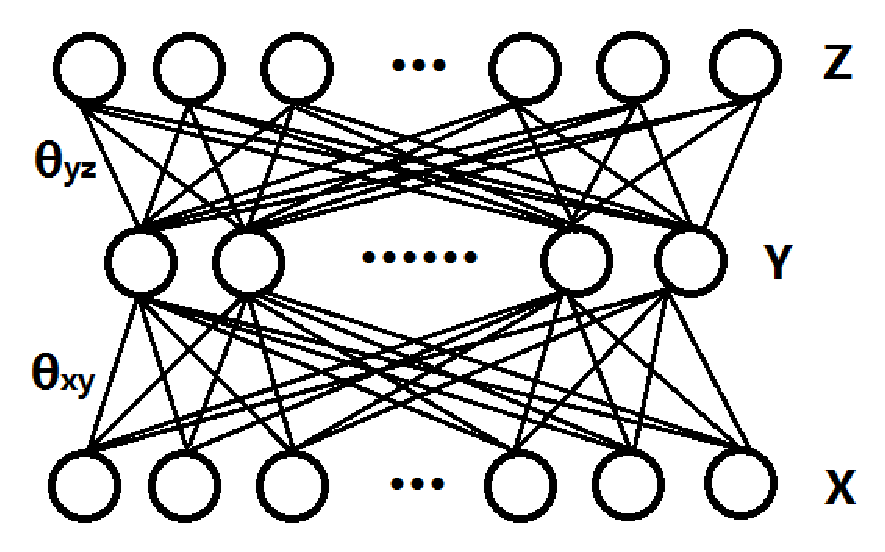
\includegraphics[width=0.4\textwidth]{3NN.eps}
\caption{三层神经网络的网路构型}
\label{img:3NN}
\end{figure}
如图中的三层神经网络,$y$层到$z$层为分类器,根据之前的讨论,我们可以利用式\eqref{equ:5.0}和式\eqref{equ:5.00} 求取$\partial J(\theta)/\partial \theta_{yz}$的值,如果我们要求取$\partial J(\theta)/\partial \theta_{xy}$的值,那么通过链式求导,我们有
\begin{equation}
\frac{\partial J(\theta)}{\partial\theta_{xy}} = \frac{\partial J(\theta)}{\partial y} \frac{\partial y}{\partial net_y} \frac{\partial net_y}{\partial \theta_{xy}}\label{equ:xxxxx}
\end{equation}
而我们又可以求得
\begin{equation}
\frac{\partial J(\theta)}{\partial y} =  \frac{\partial J(\theta)}{\partial net_z} \frac{\partial net_z}{\partial y}\label{equ:5.0.5}
\end{equation}
如果我们定义式\eqref{equ:5.0}以及式\eqref{equ:5.00}中的误差为
\begin{equation}
\delta_z = \frac{\partial J(\theta)}{\partial net_z}
\end{equation}
那么我们可以将式\eqref{equ:5.0.5}写为
\begin{equation}
\frac{\partial J(\theta)}{\partial y}  =  \delta_z \frac{\partial net_z}{\partial y} = \delta_z \theta_{yz}^T
\end{equation}
式中,$\partial J(\theta) /\partial y$就是分类器输出层(Z层)的误差传播回其上一层(Y层)的误差,如果我们定义Y层的误差为
\begin{equation}
\delta_y = \frac{\partial J(\theta)}{\partial y} \frac{\partial y}{\partial net_y}
\end{equation}
则我们可以利用后一层传播回来的误差$\delta_z$计算该层的误差
\begin{equation}
\delta_y = \delta_z \theta_{yz}^T  \cdot \frac{\partial y}{\partial net_y}
\end{equation}
从而我们可以利用该层的误差$\delta_y$计算该层参数$w_{xy}$的增量,即梯度
\begin{equation}
\frac{\partial J(\theta)}{\partial\theta_{xy}} =\delta_y \cdot  \frac{\partial net_y}{\partial \theta_{xy}}\label{equ:yyyyy}
\end{equation}
通过式\eqref{equ:yyyyy}对参数$\theta_{xy}$进行校正,校正完毕后,如果网络不止三层,而是四层,假设X层的下一层为P层,那么为了计算连接X层与P层参数$\theta_{px}$的梯度,利用链式求导,同样有
\begin{equation}
\frac{\partial J(\theta)}{\partial\theta_{px}} = \frac{\partial J(\theta)}{\partial x} \frac{\partial x}{\partial net_x} \frac{\partial net_x}{\partial \theta_{px}}\label{equ:zzz}
\end{equation}
与之前的做法类似,我们有
\begin{equation}
\begin{split}
\frac{\partial J(\theta)}{\partial x} & = \frac{\partial J(\theta)}{\partial y}  \frac{\partial y}{\partial net_y}\frac{\partial net_y}{\partial x}\\
&=\delta_y \cdot \theta_{xy}^T
\end{split}
\end{equation}
同样的道理,X层的误差$\delta_x$定义为
\begin{equation}
\delta_x =   \frac{\partial J(\theta)}{\partial x} \frac{\partial x}{\partial net_x} = \delta_y  \theta_{xy}^T \cdot \frac{\partial x}{\partial net_x}
\end{equation}
则参数$\theta_{px}$的梯度便可以利用$\delta_x$计算
\begin{equation}
\frac{\partial J(\theta)}{\partial\theta_{px}} = \delta_x \cdot \frac{\partial net_x}{\partial \theta_{px}}
\end{equation}
如果还有更多的层,其原理雷同,我们不再详细叙说。现在让我们抛开以上的数学内容从网络的结构上解释这个算法为什么叫做误差反向传播,首先我们观察各层的误差,即
\begin{equation}
[\delta_z~~\delta_y~~\delta_x ] = \bigg[~~
\frac{\partial J(\theta)}{\partial net_z}~~~~~~
\delta_z \theta_{yz}^T  \cdot \frac{\partial y}{\partial net_y}~~~~~~
\delta_y  \theta_{xy}^T \cdot \frac{\partial x}{\partial net_x}
~~\bigg]\label{equ:delta inject}
\end{equation}
式中,$\theta^T$起到的作用是将误差$\delta$反向注入的行为,这个行为如图\ref{img:3NNbp}所示
\begin{figure}[!htbp]
\centering
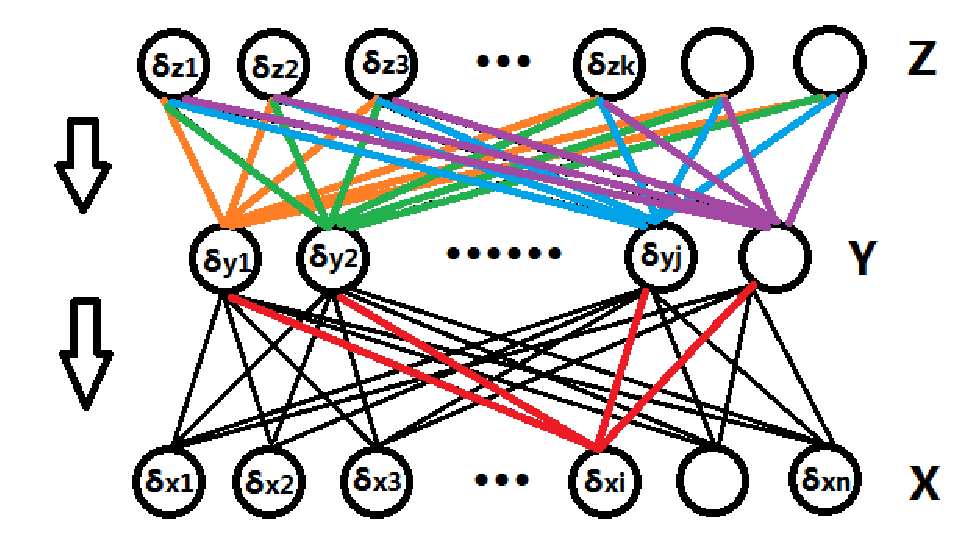
\includegraphics[width=0.55\textwidth]{DBN/3NNbp.eps}
\caption{误差反向注入}
\label{img:3NNbp}
\end{figure}

观察式\eqref{equ:delta inject},我们不难看出,除了最顶层外,剩余层的误差形式都是类似的,如果用一句话概括反向传播算法,便是:将$\ell$层的误差注入到$\ell - 1$层中,再乘上$\ell -1$层激活函数的导数,得到$\ell - 1$层的误差,利用这个得到的误差,对$\ell - 1$层的参数进行更新,更新完毕后,将$\ell - 1$层的误差重新注入到$\ell - 2$层,重复上述步骤直至误差传遍整个网络。但是这里有个例外,最顶层的误差定义与剩余层的不一样,之所以会这样是因为最顶层的误差并不是通过注入方式得到的,而是人为定义得到的,因为这个误差源自于准则函数。

我们可以看到,反向传播这种策略实际上与前向传播是类似的,反向传播也是一种贪婪算法,这将会导致一些问题。因为每一次误差传播都是更新参数后再将误差注入回前一层,这并不能保证计算得到的梯度就是真实的梯度,一旦网络的层数过深,将会导致前面层的真实导数与利用反向传播计算得到的导数相差过大。另外,如果使用sigmoid函数作为激活函数,它将很容易进入饱和状态,前面层的梯度接近于0,从而参数无法更新,这种现象我们称之为梯度消失。一种对抗梯度消失的方法是将sigmoid函数换成ReLU激活函数,关于ReLU为什么可以抵抗梯度消失的原理目前尚未研究出来,但是实验现象表明它确实能抑制梯度消失。

\BiSection{深度置信网络}
x深度置信网路(Deep Belief Networks,简写为DBN)本质就是一种传统的神经网络,但是它在传统神经网络的基础上加入一些变动。首先,这是一种深层的神经网络,而传统的神经网络一般只设计为三层结构。另外,深度置信网络是一个以受限玻尔兹曼机为基础,多个受限玻尔兹曼机垒出来的多层神经网络。图\ref{img:DBN}展示了一个深度为4的深度置信网络。
\begin{figure}[!htbp]
\centering
\includegraphics[width=0.35\textwidth]{DBN.eps}
\caption{DBN网络构型}
\label{img:DBN}
\end{figure}

我们之所以采用深度结构,是因为在神经元总数不变的前提下,深度结构的表达能力比浅结构的表达能力更强。之所以要在这个结构中引入受限玻尔兹曼机,是因为传统的深度结构无法训练。正如我们前面提及到的,深度结构会在网络的较浅层出现梯度消失现象,导致浅层无法对参数进行校正。由于数据必须从浅层神经元逐层地传播到深层神经元,一旦浅层的参数无法校正,将会导致深层的网络也无法进行参数校正,因为浅层参数无法校正意味着浅层无法对数据进行合理地重编码,数据经过浅层后得到的是混乱的数据,尽管深层不会产生太大的梯度消失现象,但数据经过浅层的打乱后,数据已经混乱了,训练也便没有意义。另一方面,传统的神经网络初始值设定为随机值,这些随机值一般设定为一个均值为0,方差较小的高斯分布,神经网络是一个非凸问题,局部最小值众多,网络最后收敛到的最小值取很大程度上决于初始值的选取,随机选取初始值虽然是一个可行的方法,但是如果我们能让参数的初始值设定在一个较合理的初始值,将会很大程度地改善网络的收敛性能,而受限玻尔兹曼机一个重要的贡献在于,将深度神经网络的参数初始化到一个较好的值。

深度置信网络的训练分为两个阶段,分别是预训练阶段和参数微调阶段。在DBN的预训练阶段中,将相邻两层看做一个受限玻尔兹曼机,采用受限玻尔兹曼机的训练方法,将原始数据作为最底层的输入,每层RBM隐含层的输出作为后一层的输入,然后进行逐层贪婪的无监督训练。对于每层RBM,其训练过程描述如算法\ref{alg:RBM} 所示

\vspace{1em}
\begin{minipage}{0.8\textwidth}\centering
\begin{algorithm}[H]\label{alg:RBM}
 \caption{受限玻尔兹曼机训练算法}
  \KwIn{由前一层网络提供的含有$n$个样本的数据集$S = \{x_i\}_{i=1}^n$;网络参数$w, b_h, b_v$; 动量项系数$p$;\\~~~~~~~~~~~~学习率$\eta$;权衰减系数$e$;CD-k中的参数$k$}
 \KwOut{训练好的网络参数;\\~~~~~~~~~~~~~~~由RBM提取到的数据$S' = \{y_i\}_{i=1}^n$}
\For{$i=1$;$i\leq1$; $i++$}
{
$v_0 = v_t = x_i$\\
$h_0$ = sampling h given v ($v_0$)\\
\For{$j=0$; $j < k$; $j++$}{
$h_t$ = sampling h given v ($v_t$)\\
$v_t $ = sampling v given h ($h_t$)\\
}
$\Delta_w = v_t^T * h_t - v_0^T * h_0$\\
$\Delta_{b_v} = v_t - v_0$\\
$\Delta_{b_h} = h_t - h_0$\\
$w = e * (p*w + \eta * \Delta_w)$\\
$b_v = b_v + \eta * \Delta_{b_v}$\\
$b_h = b_h + \eta * \Delta_{b_h}$\\
$y_i$ = sampling h given v ($x_i$)
}
\end{algorithm}
\end{minipage}
\vspace{1em}

算法中,学习率$\eta$、动量项系数$p$以及权衰减系数$e$我们将会留到网络设计技巧中讨论,这些技巧在数学推导的过程中是不必要的,然而在实际工程中是必要的,有时候缺了它们网络训练会失败。当逐层训练完毕后,网络的参数已经初始化到一个较好的位置\citeup{whyHelp}。在参数微调阶段,接着执行全局的反向传播算法进行有监督的权值微调。通过这样的方法,可以避免单纯地使用反向传播方法中会出现的陷入局部最优问题,由于识别的过程中,数据是逐层地进行维度变化,所以DBN也可以认为是一种特征提取方法,对应的,深度学习有时候也称之为“特征学习”\citeup{multipRespresen}。

\BiSection{本章小结}
x本章中,我们从传统的神经网络说起,介绍了神经元的工作原理以及神经网络的前向传播。当数据经过神经网络的逐层编码后,得到的编码并不是人类所能理解的编码,因此我们介绍了两种分类器将这些编码转换成自然语言所能描述的编码。随后我们介绍了神经网络的反向传播算法,最后引出深度置信网络。尽管这章名为“深度置信网络”,我们却对“深度置信网络”的介绍篇幅很短,但由于深度置信网络中并没有太多额外的东西,很多思想都是与传统神经网络是相同的,所以我们花了较大的篇幅取介绍传统神经网络。在本章中,我们依然留下一些问题没有解决,即训练过程中的一些额外参数,例如学习率、动量项等,关于这些内容,由于其更偏向于工程内容,我们将其集中到“神经网络设计技巧”章节中讨论。



